% Chapter Template

\chapter{Ensayos y resultados} % Main chapter title

\label{Chapter4} % Change X to a consecutive number; for referencing this chapter elsewhere, use \ref{ChapterX}


%----------------------------------------------------------------------------------------
%	SECTION 1
%----------------------------------------------------------------------------------------
En este capítulo se detallan los resultados esperados y obtenidos sobre cada una de las pruebas realizadas para validar la integración del sistema y poder comprobar que el alcance funcional logrado es acorde a los esperado.

%\citep{ARTICLE:1}, \citep{BOOK:1}, \citep{BOOK:2}, \citep{WEBSITE:1}.

\section{Banco de pruebas}

Todos los ensayos que se describen en este capítulo fueron efectuados utilizando el diseño físico de red que se muestra en la figura \ref{fig:banco}. Las pruebas funcionales desde dentro de la red local se realizaron con una laptop MacBook Pro y un equipo de escritorio con Windows 10. Para las pruebas de funcionalidad remota se realizaron utilizando un dispositivo móvil Samsung A50 con acceso a la red celular mediante el uso de paquetes de datos a Internet.

\begin{figure}[htbp]
	\centering
	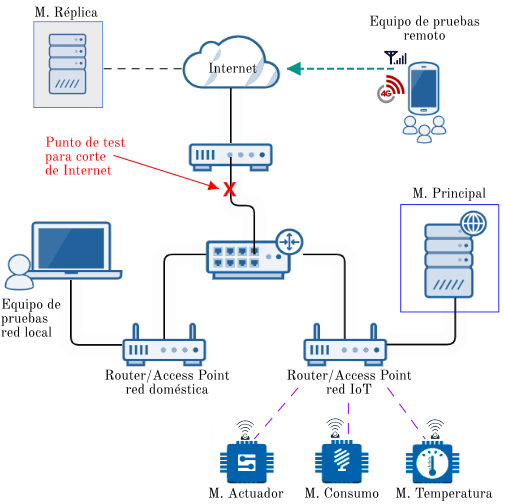
\includegraphics[width=0.91\textwidth]{./Figures/banco2.png}
	\caption{Esquema del banco de pruebas utilizado.}

	\label{fig:banco}
\end{figure}


\section{Resultados de los módulos del sistema IoT}
En esta sección se muestran las imágenes reales de los resultados obtenidos de la construcción de cada módulo físico. Estos dispositivos fueron utilizados para las pruebas de validación en un ambiente real IoT. Las figuras \ref{fig:modPrincipal}, \ref{fig:modTemp} y \ref{fig:modConsumo2} muestran los módulos.

 
\begin{figure}[htpb]
\centering 
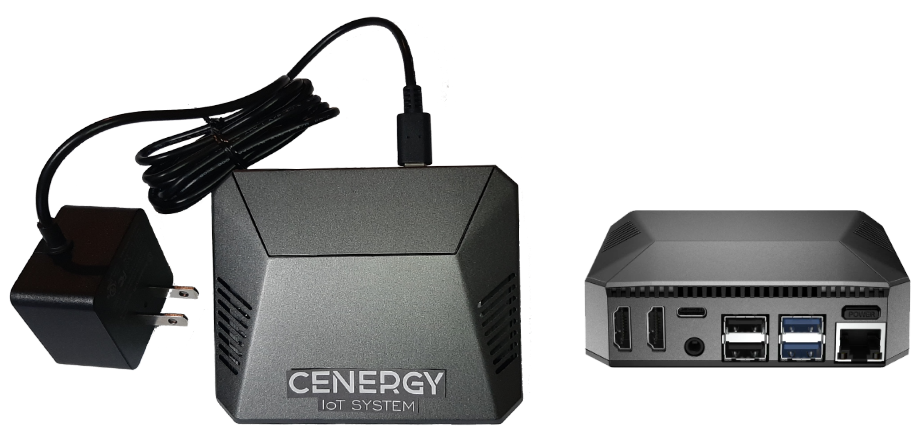
\includegraphics[width=0.95\textwidth]{./Figures/principal2.png}
\caption{Vista superior y posterior del módulo principal.}
\label{fig:modPrincipal}
\end{figure}



\begin{figure}[htpb]
\centering 
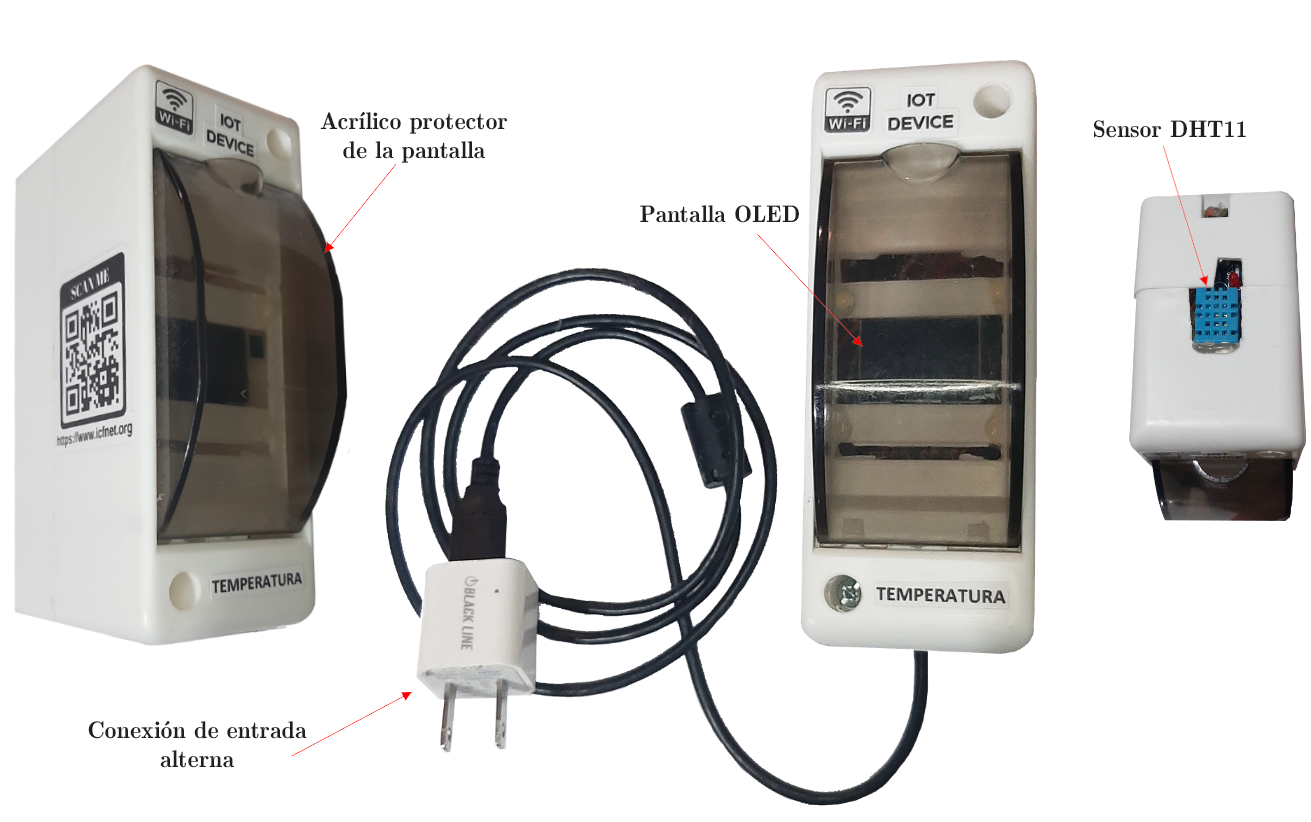
\includegraphics[width=0.9\textwidth]{./Figures/moduloTemp.png}
\caption{Vista lateral, frente y superior del módulo de temperatura.}
\label{fig:modTemp}
\end{figure}



%%%%%%%%%%%%%%%%%%%%%%%%%%%%%%%%%%%%%%%%%%%%%%%%%%%

\begin{landscape} % esto es para rotar la pagina e imagen
\begin{figure}[htpb]
\centering 
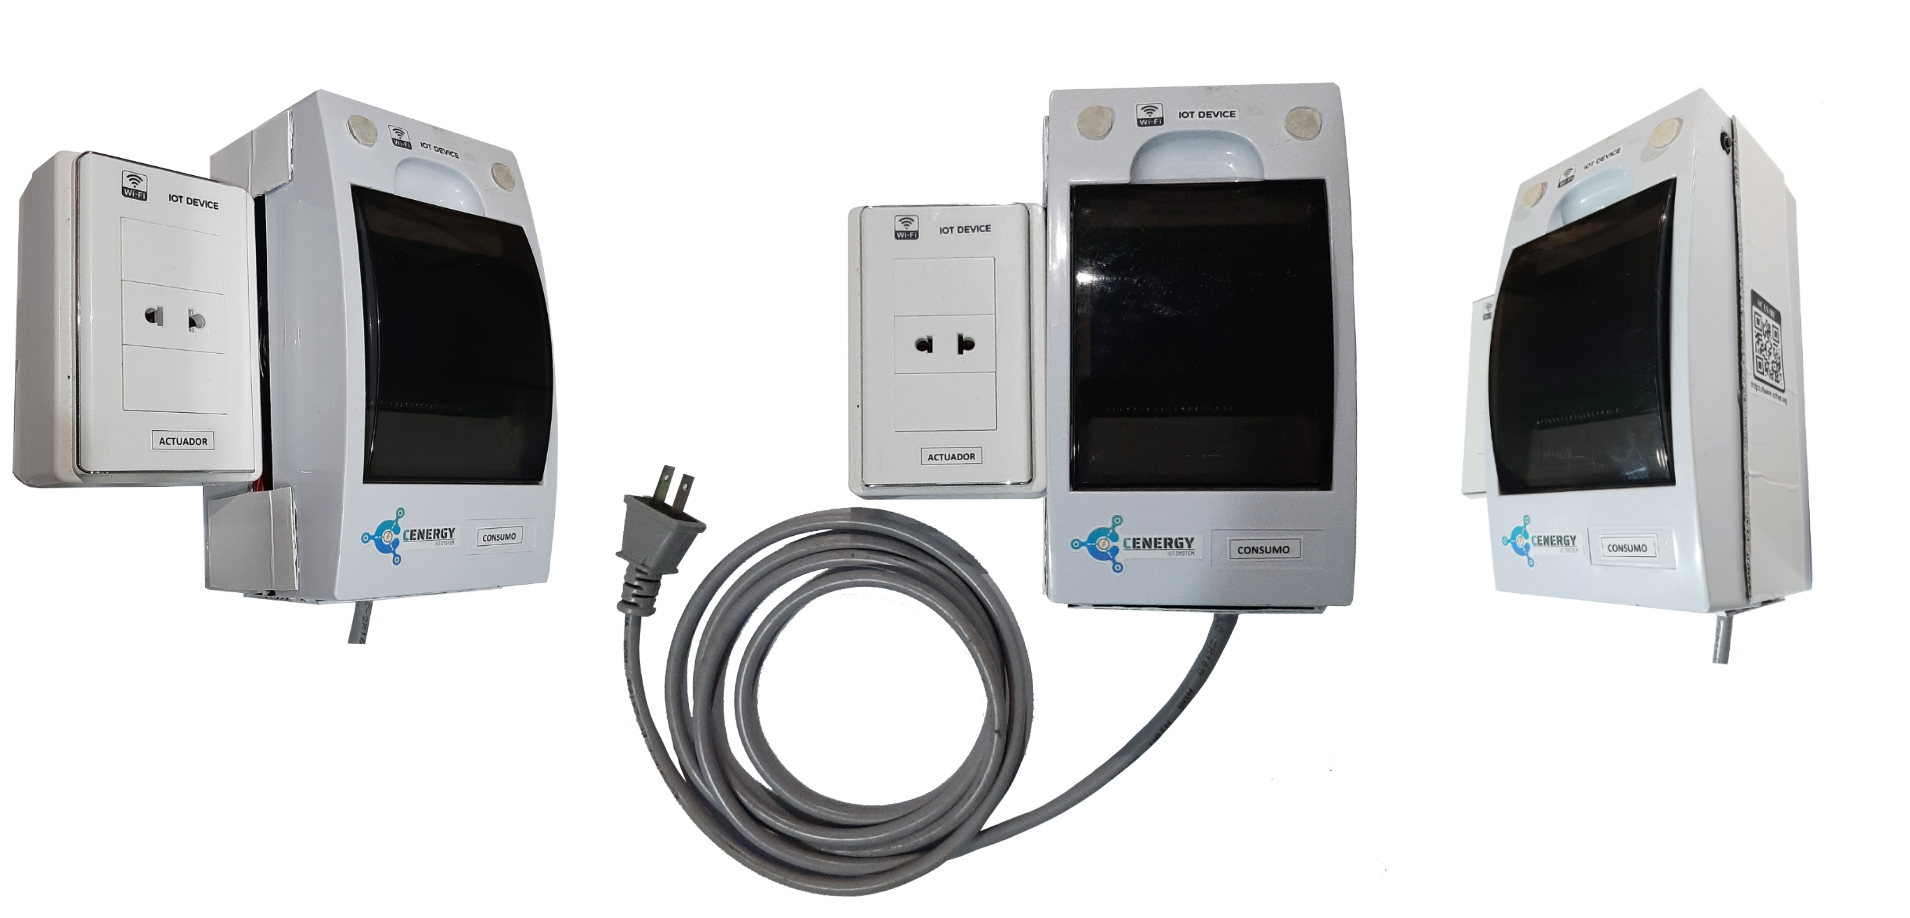
\includegraphics[width=1.8\textwidth]{./Figures/consumo2.png}
\caption{Vista frontal y lateral del módulo actuador y módulo de consumo.}
\label{fig:modConsumo2}
\end{figure}
\end{landscape} %


%%%%%%%%%%%%%%%%%%%%%%%%%%%%%%%%%%%%%%%%%%%%%%%%%%%
\section{Interfaces gráficas del software de monitoreo}

El software de monitoreo y control fue diseñado y desarrollado a medida con el objetivo de ser el autor de este trabajo el dueño de los derechos de \emph{Copyright} del mismo, ademas el software por ser de tipo web requiere solo un navegador web y estar conectado a la red local o a Internet para poder ser utilizado. El software ha sido nombrado como: \emph{Cenergy IoT System} y hace referencia al control de energía eléctrica mediante un sistema IoT. Se espera su evolución y madurez en trabajos futuros.

Las principales interfaces gráficas de usuario (GUI) que se muestran a continuación son el resultado de lo logrado en esta primera version del software hasta la fecha de presentación de este trabajo. Las GUIs son:

\begin{itemize}
\item La interfaz de control de acceso al sistema se muestra en la figura \ref{fig:gui0}. Los credenciales utilizados son el numero de su documento nacional de identidad (DNI)y una contraseña de longitud mínima de 8 caracteres.

\item La interfaz de presentación inicial al ingresar al sistema (dashboard) se muestra en la figura \ref{fig:gui1}. Esta interfaz muestra el resumen de lo que actualmente esta almacenado en la base de datos del sistema. Resalta el consumo facturado y el no facturado a la fecha actual de acceso considerando intervalos de un mes.

\item La interfaz de monitoreo para sensores se muestra en la figura \ref{fig:gui2}. Esta interfaz permite mostrar en tiempo real los sensores que tiene el sistema IoT, así como el estado de los mismos. 

Si un sensor tiene un estado CONECTADO se podrá observar sus detalles desde la opción ``ver detalles'', pudiendo acceder a una vista gráfica más detallada del mismo, tal como se muestra en la figura \ref{fig:gui2-1}.

\item La interfaz de monitoreo y control para sensores de consumo y sus actuadores se muestran el figura \ref{fig:gui3}. Esta interfaz permite visualizar en tiempo real los módulos registrados y conectados al sistema IoT.

Cada módulo en estado CONECTADO muestra el dispositivo que esta realizando consumo mediante una onda de señal de energía activa, junto a su interruptor actuador cuya función es el control del paso o limitación de energía eléctrica en el módulo.

Si el módulo esta con el estado CONECTADO se podrá observar sus detalles desde la opción ``ver detalles'', pudiendo acceder a una vista gráfica más detallada del mismo, tal como se muestra en la figura \ref{fig:gui3-1}.

\item La interfaz de registro o agregado de módulos al sistema IoT se muestra en la figura \ref{fig:gui4}. Para el registro cada módulo cuenta con un código y numero de módelo, para su identificación dentro del sistema.

\item El software actualmente presenta interfaces para cuatro tipos de consultas, que son: lecturas de temperatura, historial de temperatura, consumo sin facturar y consumo facturado. Cada lectura que se registra en la base de datos se respalda en agrupaciones de intervalos de horas y los registros que aun no completan las horas, podran ser consultados desde las opciones: lectura de temperatura y consumos sin facturar.

Los resultados de las búsquedas podrán ser exportados en formatos excel o pdf y si se desea, ser impresos directamente. La figura \ref{fig:gui5} muestra la interfaz de consultas.

\end{itemize}






%%%%%%%%%%%%%%%%%%%%%%%%%%%%%%%%%%%%%%%%%%%%%%%%%%%
\begin{landscape} % esto es para rotar la pagina e imagen
\begin{figure}[htpb]
\centering 
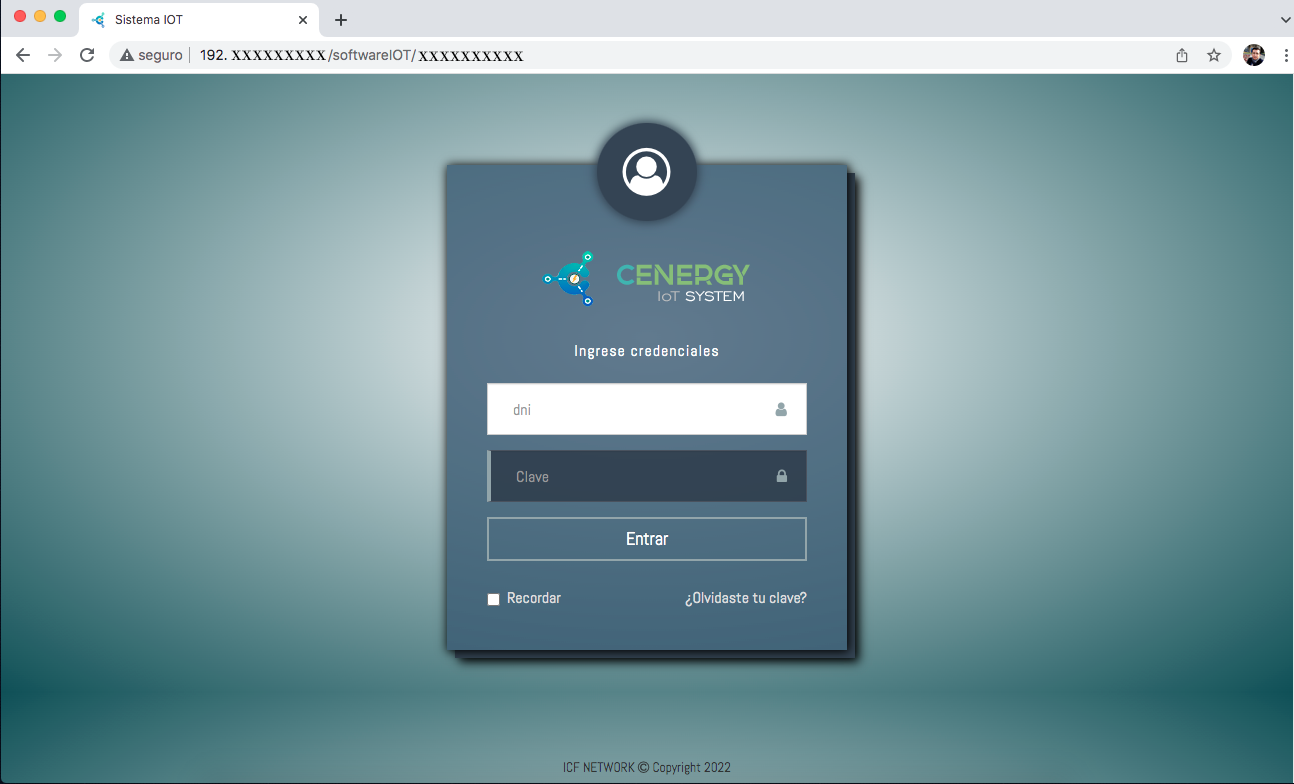
\includegraphics[width=1.55\textwidth]{./Figures/gui/0.png}
\caption{Interfaz gráfica de usuario de acceso al software de monitoreo y control.}
\label{fig:gui0}
\end{figure}
\end{landscape} %

%%%%%%%%%%%%%%%%%%%%%%%%%%%%%%%%%%%%%%%%%%%%%%%%%%%

%%%%%%%%%%%%%%%%%%%%%%%%%%%%%%%%%%%%%%%%%%%%%%%%%%%
\begin{landscape} % esto es para rotar la pagina e imagen
\begin{figure}[htpb]
\centering 
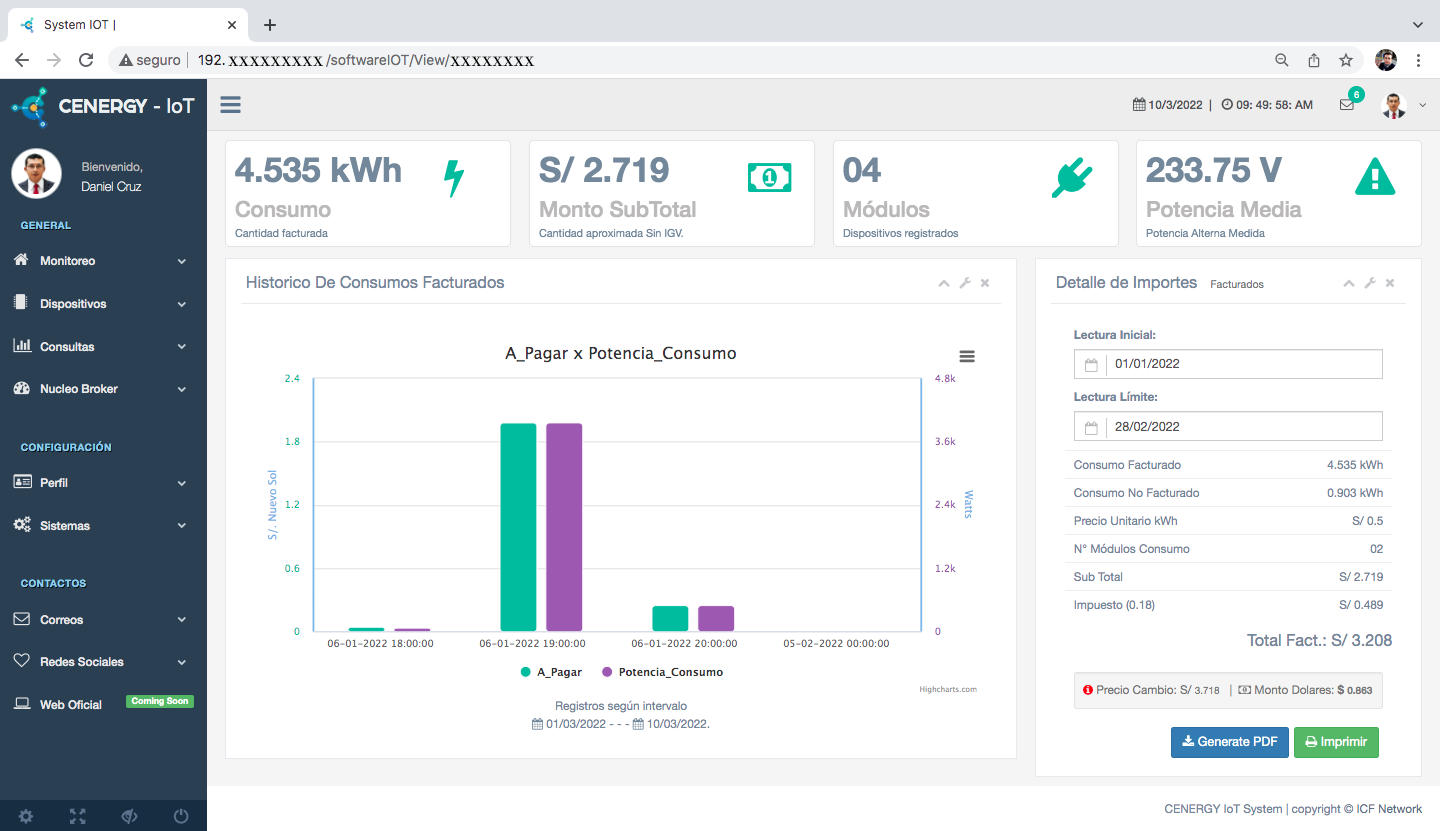
\includegraphics[width=1.55\textwidth]{./Figures/gui/1.png}
\caption{Dashboard inicial del software de monitoreo y control.}
\label{fig:gui1}
\end{figure}
\end{landscape} %

%%%%%%%%%%%%%%%%%%%%%%%%%%%%%%%%%%%%%%%%%%%%%%%%%%%

%%%%%%%%%%%%%%%%%%%%%%%%%%%%%%%%%%%%%%%%%%%%%%%%%%%
\begin{landscape} % esto es para rotar la pagina e imagen
\begin{figure}[htpb]
\centering 
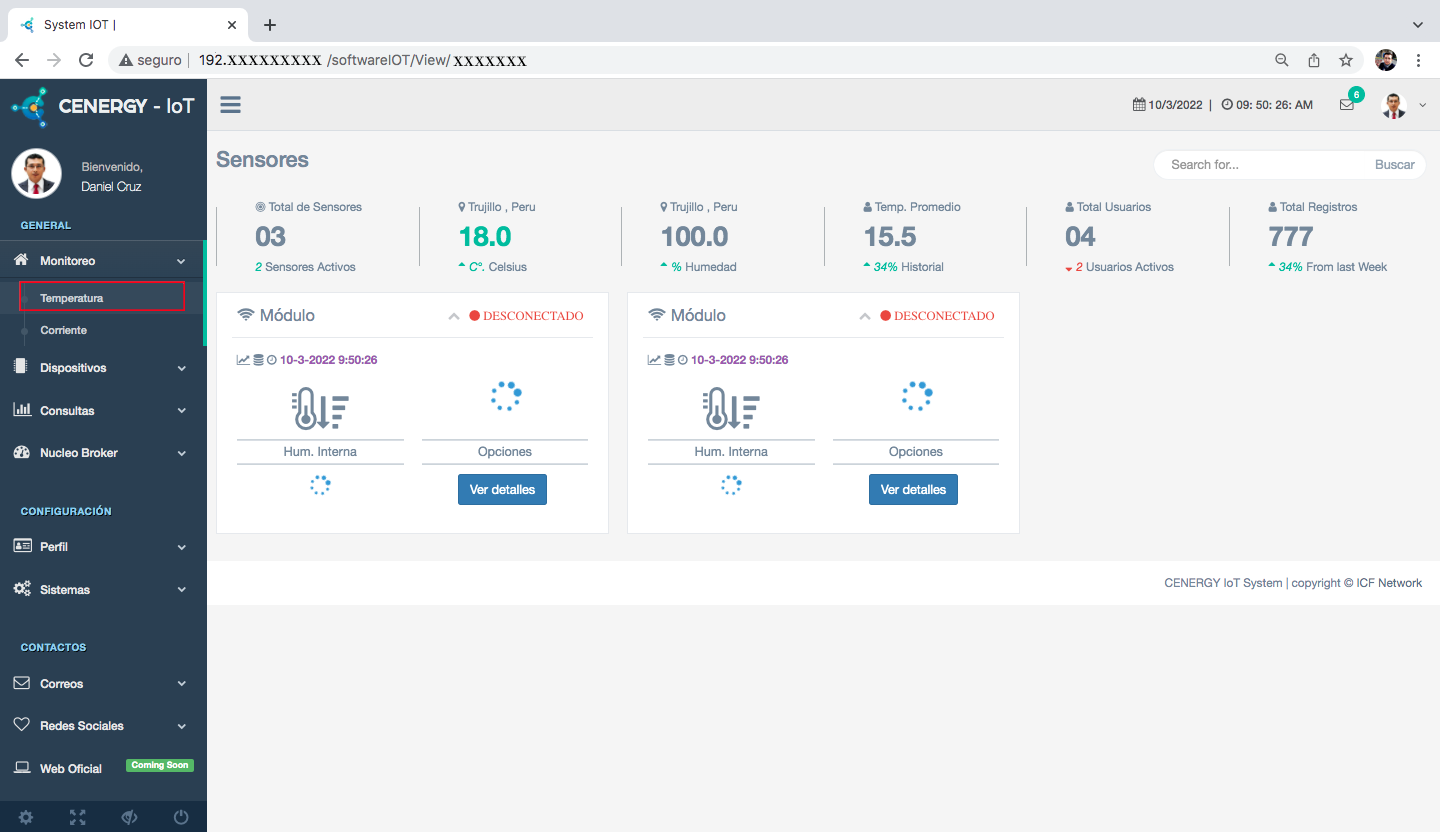
\includegraphics[width=1.55\textwidth]{./Figures/gui/2.png}
\caption{Interfaz gráfica de usuario donde se listan los sensores del sistema.}
\label{fig:gui2}
\end{figure}
\end{landscape} %

%%%%%%%%%%%%%%%%%%%%%%%%%%%%%%%%%%%%%%%%%%%%%%%%%%%

%%%%%%%%%%%%%%%%%%%%%%%%%%%%%%%%%%%%%%%%%%%%%%%%%%%
\begin{landscape} % esto es para rotar la pagina e imagen
\begin{figure}[htpb]
\centering 
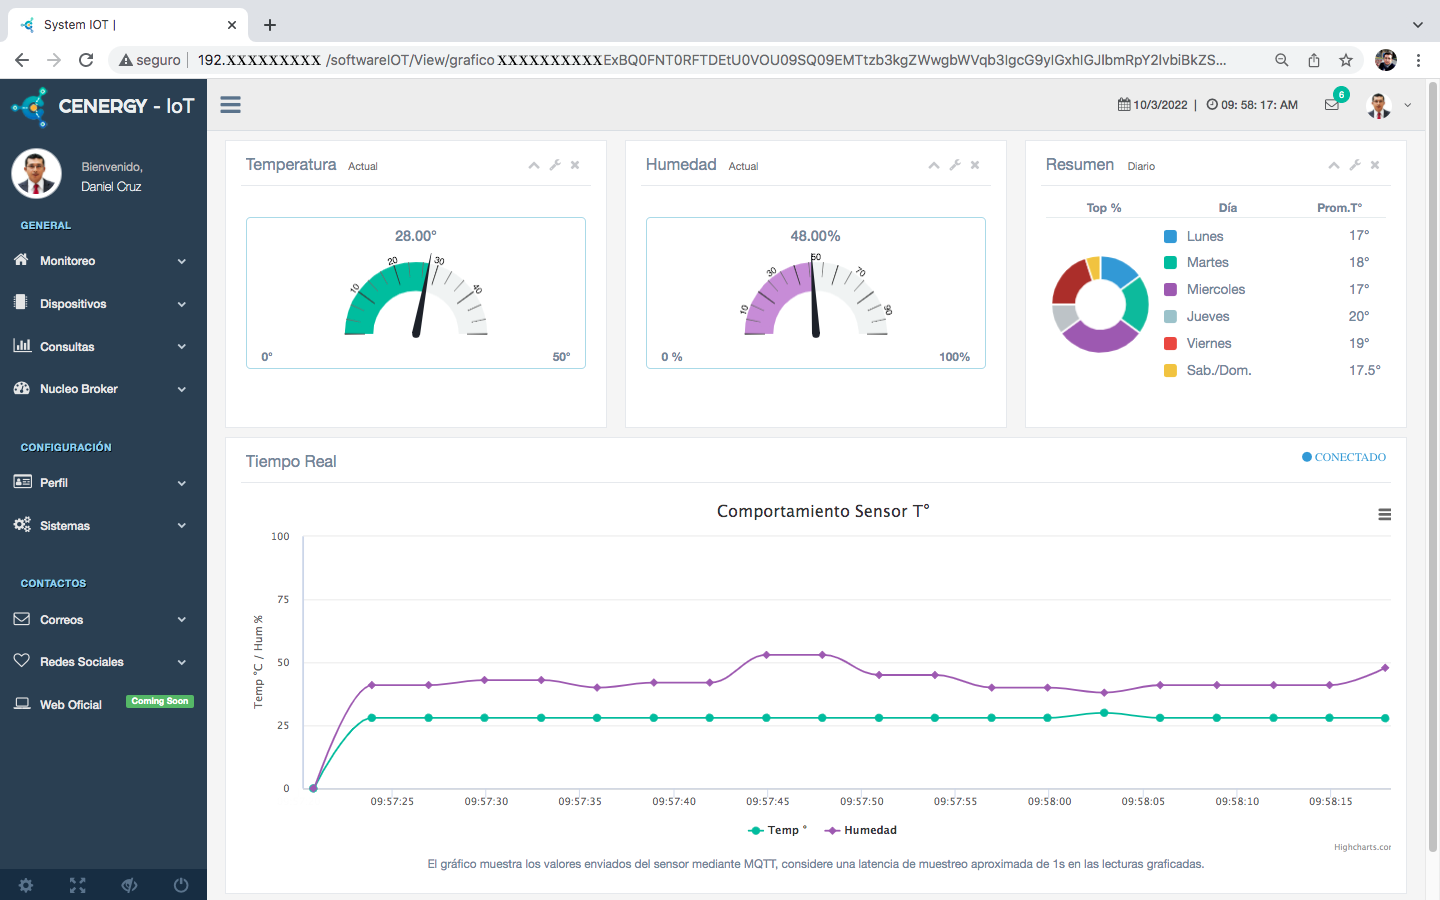
\includegraphics[width=1.5\textwidth]{./Figures/gui/2-1.png}
\caption{Interfaz gráfica de usuario donde se muestran todos los detalles de un sensor.}
\label{fig:gui2-1}
\end{figure}
\end{landscape} %

%%%%%%%%%%%%%%%%%%%%%%%%%%%%%%%%%%%%%%%%%%%%%%%%%%%

%%%%%%%%%%%%%%%%%%%%%%%%%%%%%%%%%%%%%%%%%%%%%%%%%%%
\begin{landscape} % esto es para rotar la pagina e imagen
\begin{figure}[htpb]
\centering 
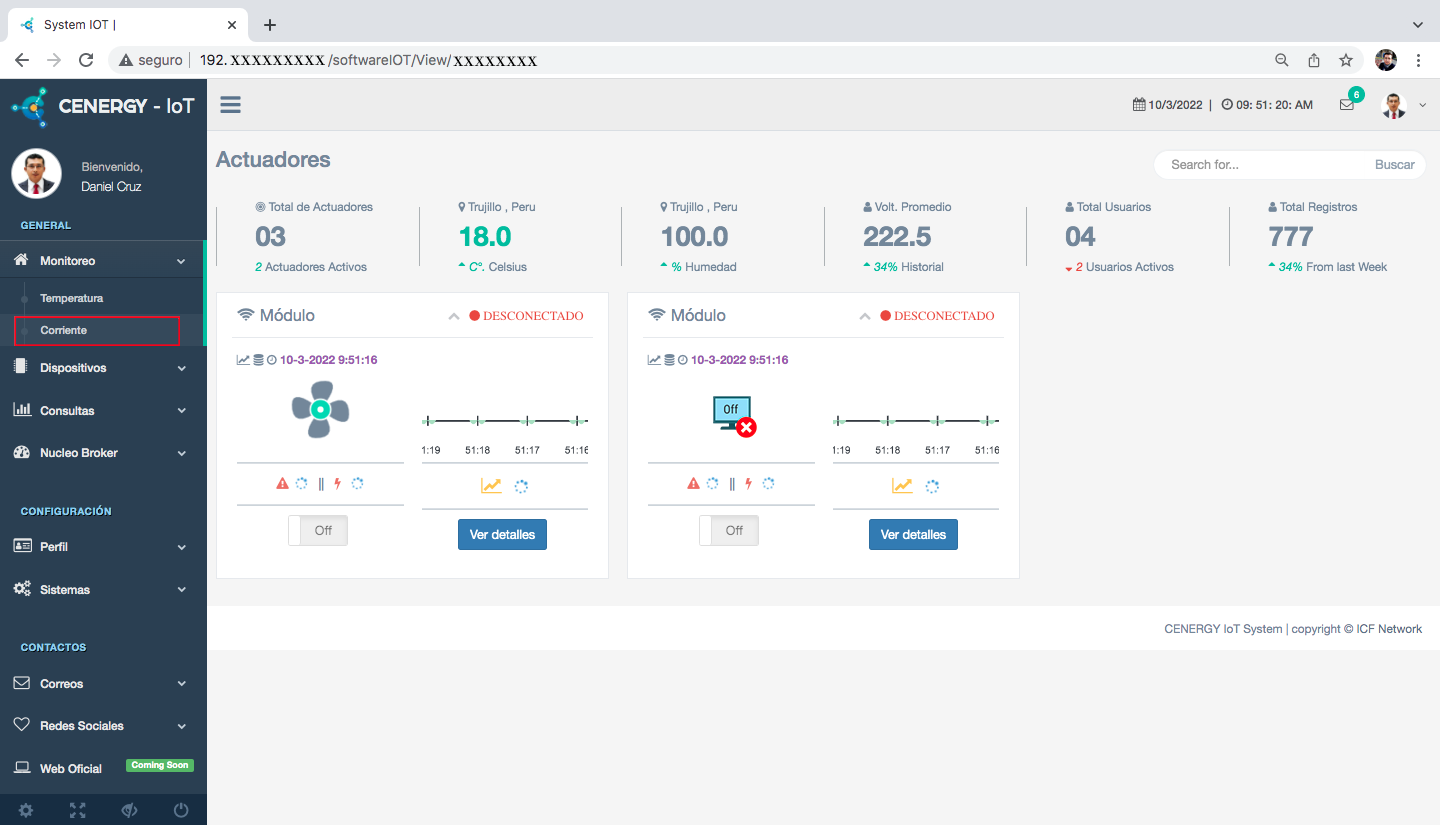
\includegraphics[width=1.52\textwidth]{./Figures/gui/3.png}
\caption{Interfaz gráfica de usuario donde se listan los sensores de consumo junto a su función de actuador.}
\label{fig:gui3}
\end{figure}
\end{landscape} %

%%%%%%%%%%%%%%%%%%%%%%%%%%%%%%%%%%%%%%%%%%%%%%%%%%%

%%%%%%%%%%%%%%%%%%%%%%%%%%%%%%%%%%%%%%%%%%%%%%%%%%%
\begin{landscape} % esto es para rotar la pagina e imagen
\begin{figure}[htpb]
\centering 
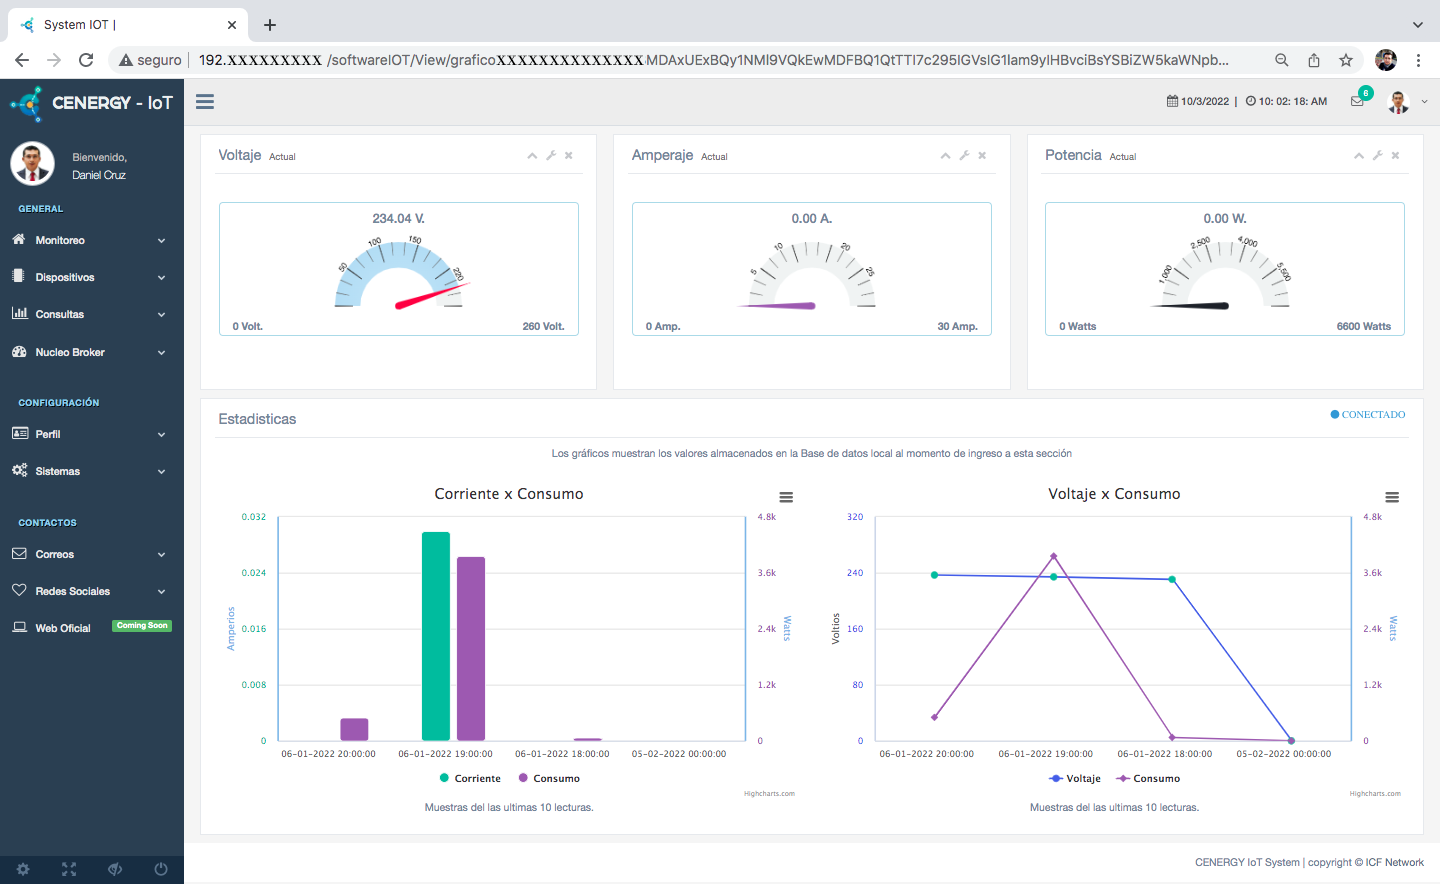
\includegraphics[width=1.52\textwidth]{./Figures/gui/3-1.png}
\caption{Interfaz gráfica de usuario donde se muestran todos los detalles de un sensor de consumo.}
\label{fig:gui3-1}
\end{figure}
\end{landscape} %

%%%%%%%%%%%%%%%%%%%%%%%%%%%%%%%%%%%%%%%%%%%%%%%%%%%

%%%%%%%%%%%%%%%%%%%%%%%%%%%%%%%%%%%%%%%%%%%%%%%%%%%
\begin{landscape} % esto es para rotar la pagina e imagen
\begin{figure}[htpb]
\centering 
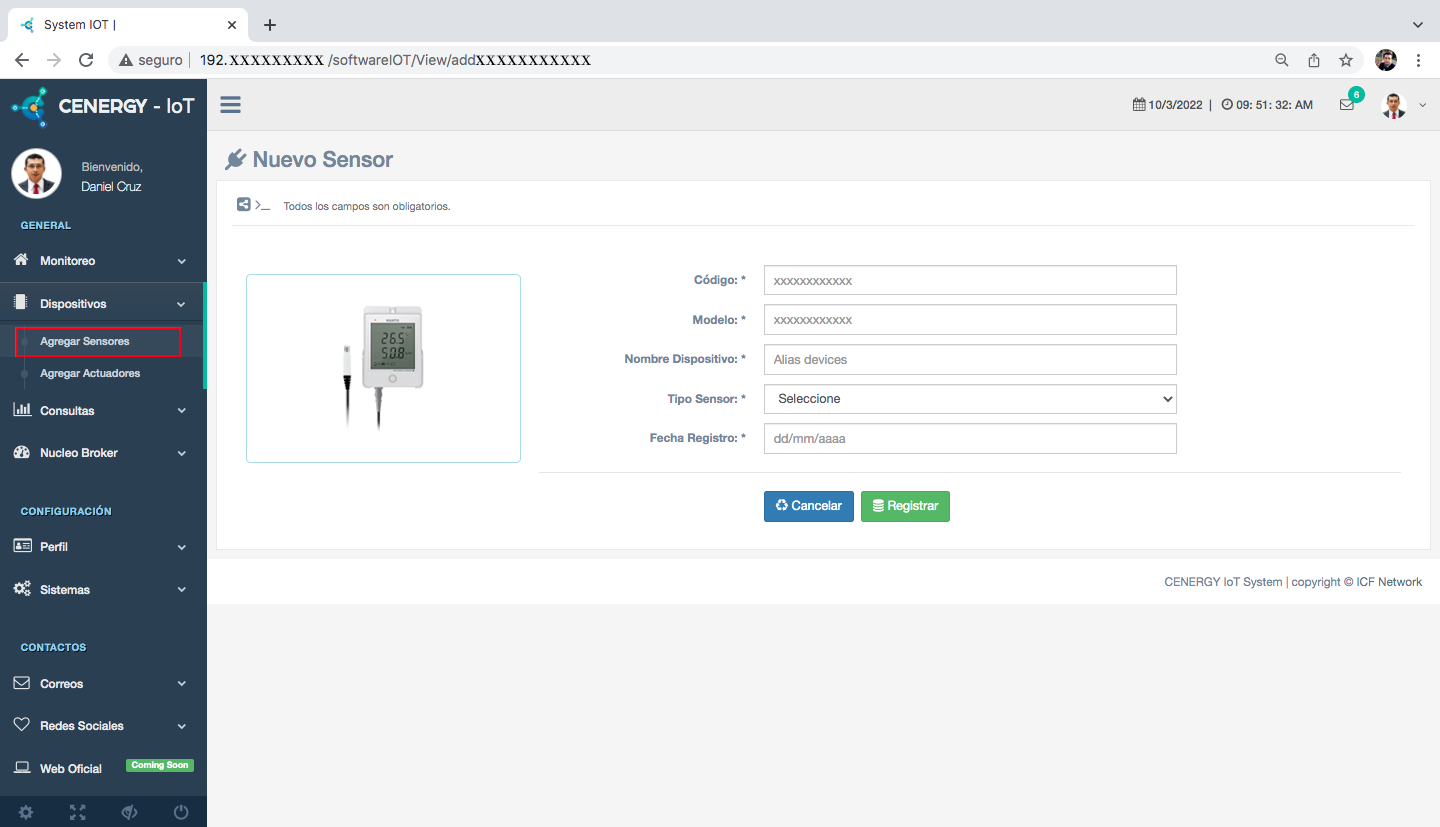
\includegraphics[width=1.55\textwidth]{./Figures/gui/4.png}
\caption{Interfaz gráfica de usuario para agregar un nuevo dispositivo al sistema.}
\label{fig:gui4}
\end{figure}
\end{landscape} %

%%%%%%%%%%%%%%%%%%%%%%%%%%%%%%%%%%%%%%%%%%%%%%%%%%%

%%%%%%%%%%%%%%%%%%%%%%%%%%%%%%%%%%%%%%%%%%%%%%%%%%%
\begin{landscape} % esto es para rotar la pagina e imagen
\begin{figure}[htpb]
\centering 
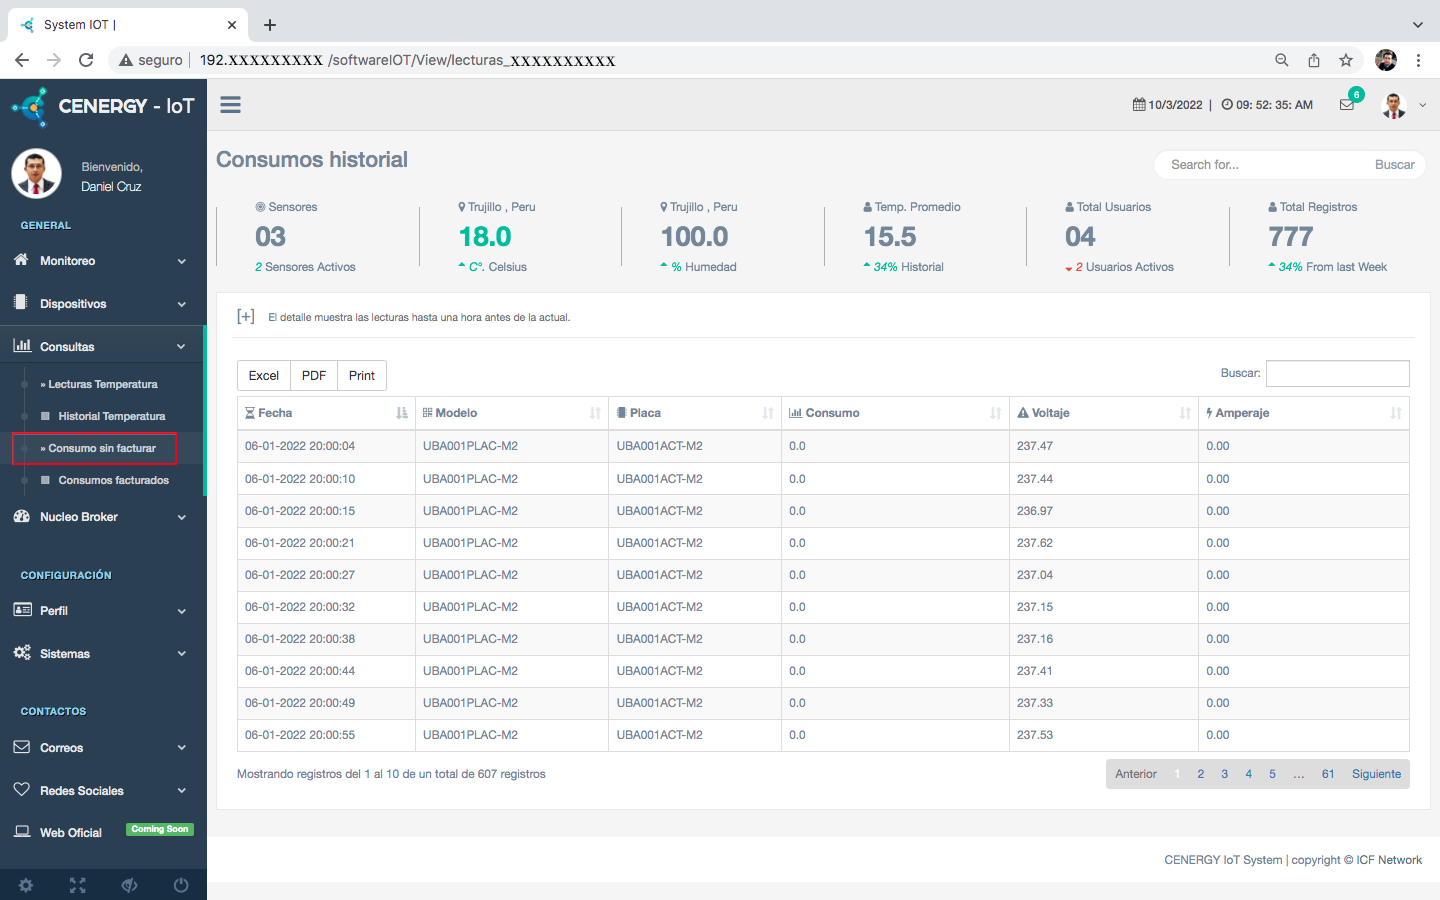
\includegraphics[width=1.5\textwidth]{./Figures/gui/5.png}
\caption{Interfaz gráfica de usuario donde se muestran las consultas y reportes de la base de datos.}
\label{fig:gui5}
\end{figure}
\end{landscape} %

%%%%%%%%%%%%%%%%%%%%%%%%%%%%%%%%%%%%%%%%%%%%%%%%%%%

\section{Pruebas de elección de canal y ancho de banda}
Para las pruebas y análisis de las señales inalámbricas se utilizó el software WiFi Explorer Lite. Es una herramienta de descubrimiento de redes inalámbricas que ayuda a identificar conflictos de canales y problemas de configuración y  pueden afectar la conectividad o el rendimiento de la red Wi-Fi de un hogar u oficina \citep{WEBSITE:24}. 

Los fundamentos y consideraciones para la elección del canal y ancho de banda de la señal Wi-Fi IoT que se utilizó, se describió en el capitulo 3. La elección dependió de las señales circundantes vecinas a la red domestica donde se instaló el sistema prototipo IoT. La figura \ref{fig:test01} muestra resultado del primer escaneo de las señales y el uso de los canales respectivos así como solapamiento existente entre ellos. 

De la figura \ref{fig:test01} se describe lo siguiente:

\keyword{Señal WLAN IoT} 
\begin{itemize}
\item SSID: MATRIX-ICF
\item Canal: 10 (configuración automática)
\item Ancho de canal: 40 MHz (configuración automática)
\item Potencia señal: 93\%
\item Seguridad:  WPA2 (PSK)
\item Tasa máxima de transferencia: 300 Mbps
\end{itemize}


\keyword{Señal WLAN doméstica}
\begin{itemize} 
\item SSID: CLARO-B612-D514
\item Canal: 11 (configuración automática)
\item Ancho de canal: 20 MHz (configuración automática)
\item Potencia señal: 64\%
\item Seguridad: WPA2 (PSK)
\item Tasa Máxima de transferencia: 144.4 Mbps
\end{itemize}

El procedimiento de mejora de la configuración de la señal IoT consistió en modificar la configuración por defecto del router/AP al cambiar el canal y reducir el ancho de banda, verificando en cada cambio el comportamiento de las señales en el ambiente y la reducción de solapamiento de los mismos.

La figura \ref{fig:test02} muestra el ancho de banda que ocupa el canal de comunicación de la señal del router sin configurar. Esta configuración por defecto demuestra no ser la más adecuada para el ambiente IoT, debido a que produce interferencias a las señales circundantes.

La figura \ref{fig:test03} muestra las características de la señal inalámbrica doméstica del lugar donde se implanto el sistema IoT prototipo.


%%%%%%%%%%%%%%%%%%%%%%%%%%%%%%%%%%%%%%%%%%%%%%%%%%%
\begin{landscape} % esto es para rotar la pagina e imagen
\begin{figure}[htpb]
\centering 
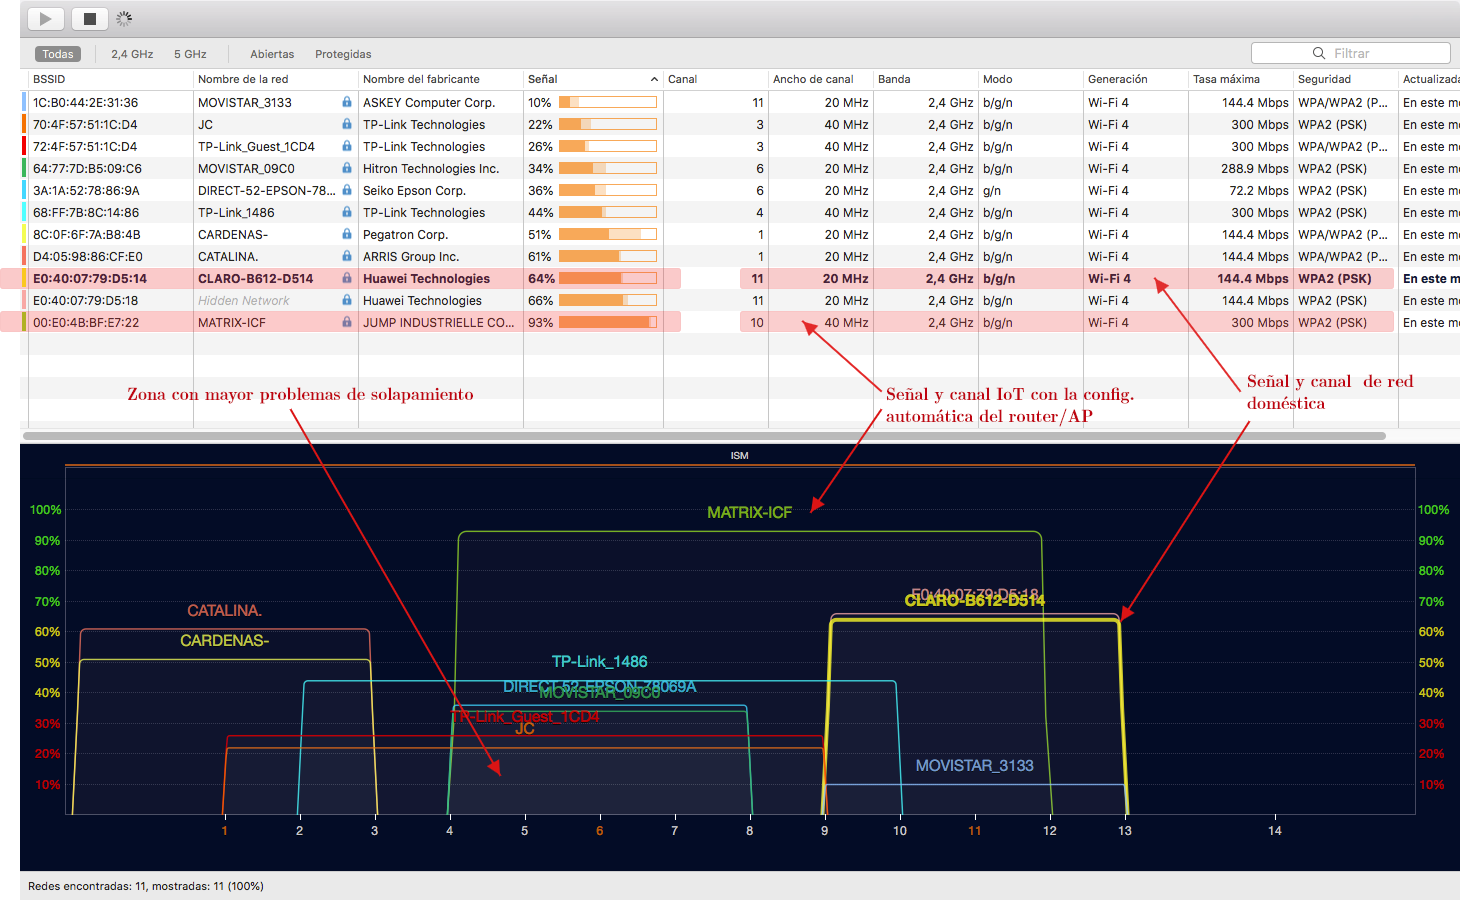
\includegraphics[width=1.5\textwidth]{./Figures/wifi/01.png}
\caption{Estado inicial de las señales Wi-Fi local y circundantes en el ambiente donde se implanto el sistema IoT.}
\label{fig:test01}
\end{figure}
\end{landscape} %

%%%%%%%%%%%%%%%%%%%%%%%%%%%%%%%%%%%%%%%%%%%%%%%%%%%

\begin{landscape} % esto es para rotar la pagina e imagen
\begin{figure}[htpb]
\centering 
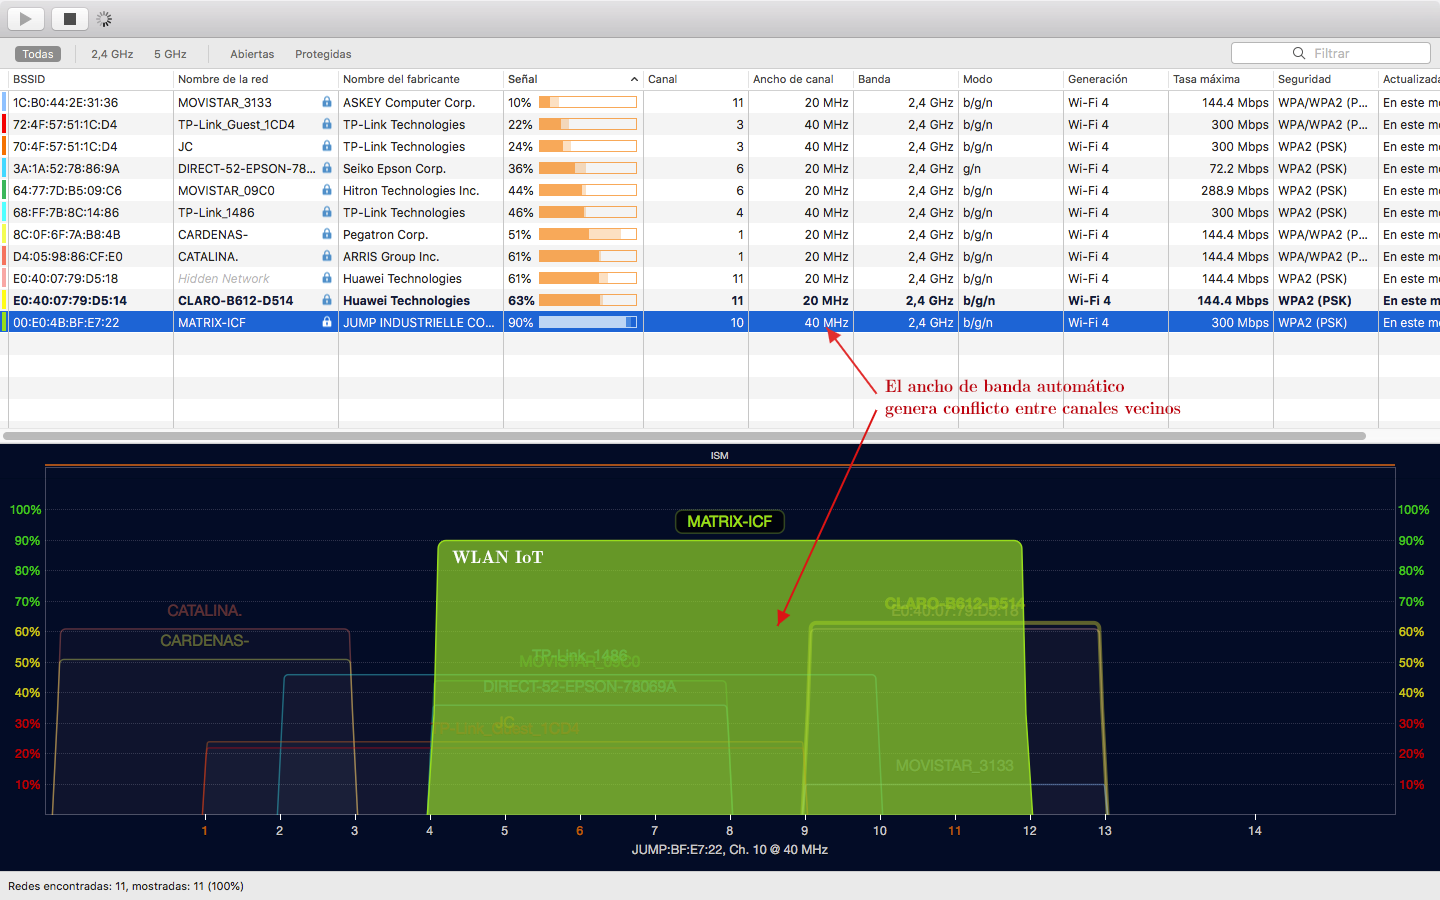
\includegraphics[width=1.5\textwidth]{./Figures/wifi/02.png}
\caption{Ancho de banda de la señal del router para la red IoT con la configuración por defecto del dispositivo.}
\label{fig:test02}
\end{figure}
\end{landscape} %


%%%%%%%%%%%%%%%%%%%%%%%%%%%%%%%%%%%%%%%%%%%%%%%%%%%
\begin{landscape} % esto es para rotar la pagina e imagen
\begin{figure}[htpb]
\centering 
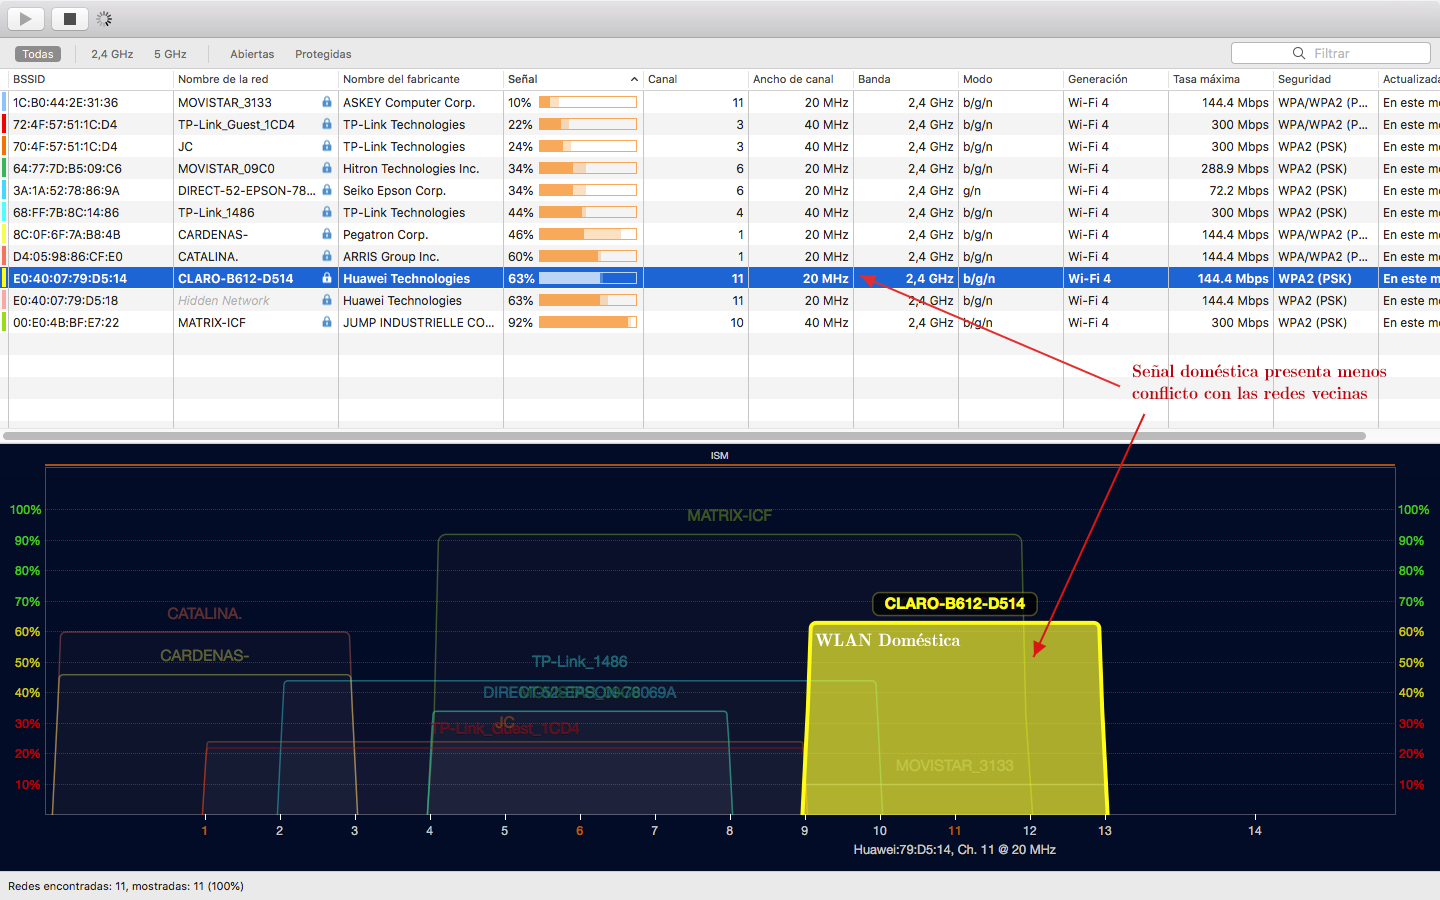
\includegraphics[width=1.5\textwidth]{./Figures/wifi/03.png}
\caption{Ancho de banda  y canal de la señal Wi-Fi doméstica.}
\label{fig:test03}
\end{figure}
\end{landscape} %

%%%%%%%%%%%%%%%%%%%%%%%%%%%%%%%%%%%%%%%%%%%%%%%%%%%%%%%%%%%%%%
El objetivo de usar un software de exploración Wi-Fi es detectar las zonas y canales con mayor interferencia y evitar que el canal elegido para nuestro trabajo tenga la mínima o ninguna intersección con la zona critica. El software detectó la zona con mayor solapamiento y lo marcó en color rojo, como se muestra en la figura \ref{fig:test04}, asociado al SSID y canal que lo causa.

El análisis de las imágenes de señales que genera el software de exploración, nos permitió conocer cuales podrían ser los canales mas ideales. Cambiar el numero de canal así como el ancho de banda del mismo, tiene como objetivo reducir o eliminar problemas de solapamiento en el canal inalámbrico usado para la red IoT. El resultado del cambio de canal para la señal destinada a la comunicación IoT, se muestra en la figura \ref{fig:test05}. 

Si se compara la figura \ref{fig:test02} (antes) con la figura \ref{fig:test05} (después), se puede observar la diferencia del canal configurado al mostrar la reducción de interferencias con las señales circundantes.

Al cambiar el canal de la señal IoT, el software cambia el color de la zona crítica (de rojo a naranja) en señal que el solapamiento se redujo, demostrando que existe una mejora en la señal de comunicación a utilizar. La figura \ref{fig:test06} muestra los resultados de mejora obtenidos.

Las pruebas y cambios de canal para el router/AP se debe realizar durante la instalación y puesta en marcha al sistema IoT y podrá ser actualizado de acuerdo al cronograma establecido para su mantenimiento. 


%%%%%%%%%%%%%%%%%%%%%%%%%%%%%%%%%%%%%%%%%%%%%%%%%%%

\begin{landscape} % esto es para rotar la pagina e imagen
\begin{figure}[htpb]
\centering 
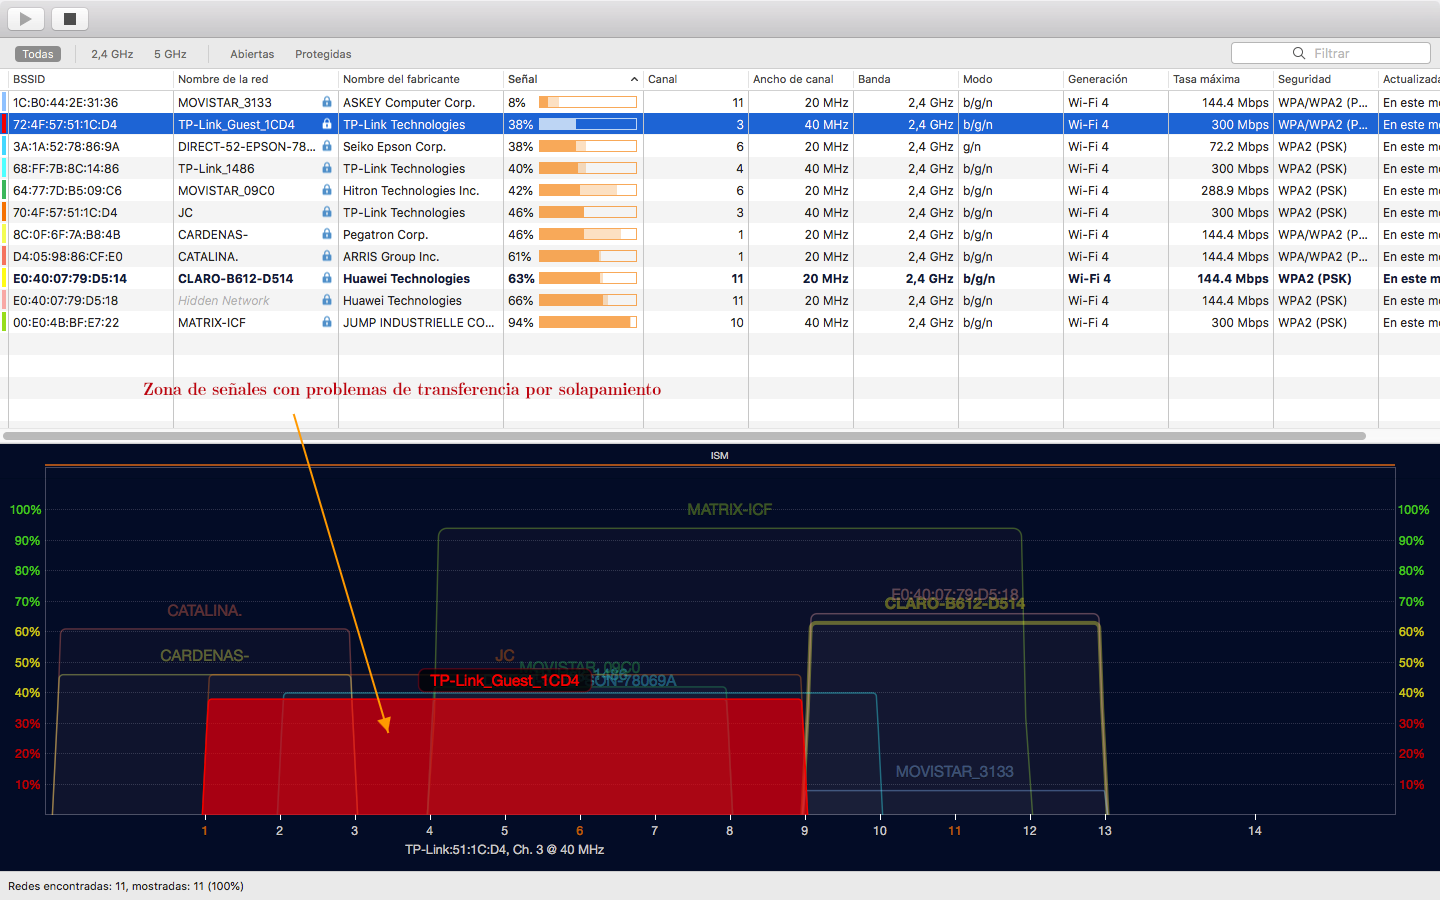
\includegraphics[width=1.5\textwidth]{./Figures/wifi/04.png}
\caption{Zona crítica con mayor interferencia entre los canales de las redes inalámbricas.}
\label{fig:test04}
\end{figure}
\end{landscape} %


%%%%%%%%%%%%%%%%%%%%%%%%%%%%%%%%%%%%%%%%%%%%%%%%%%%

\begin{landscape} % esto es para rotar la pagina e imagen
\begin{figure}[htpb]
\centering 
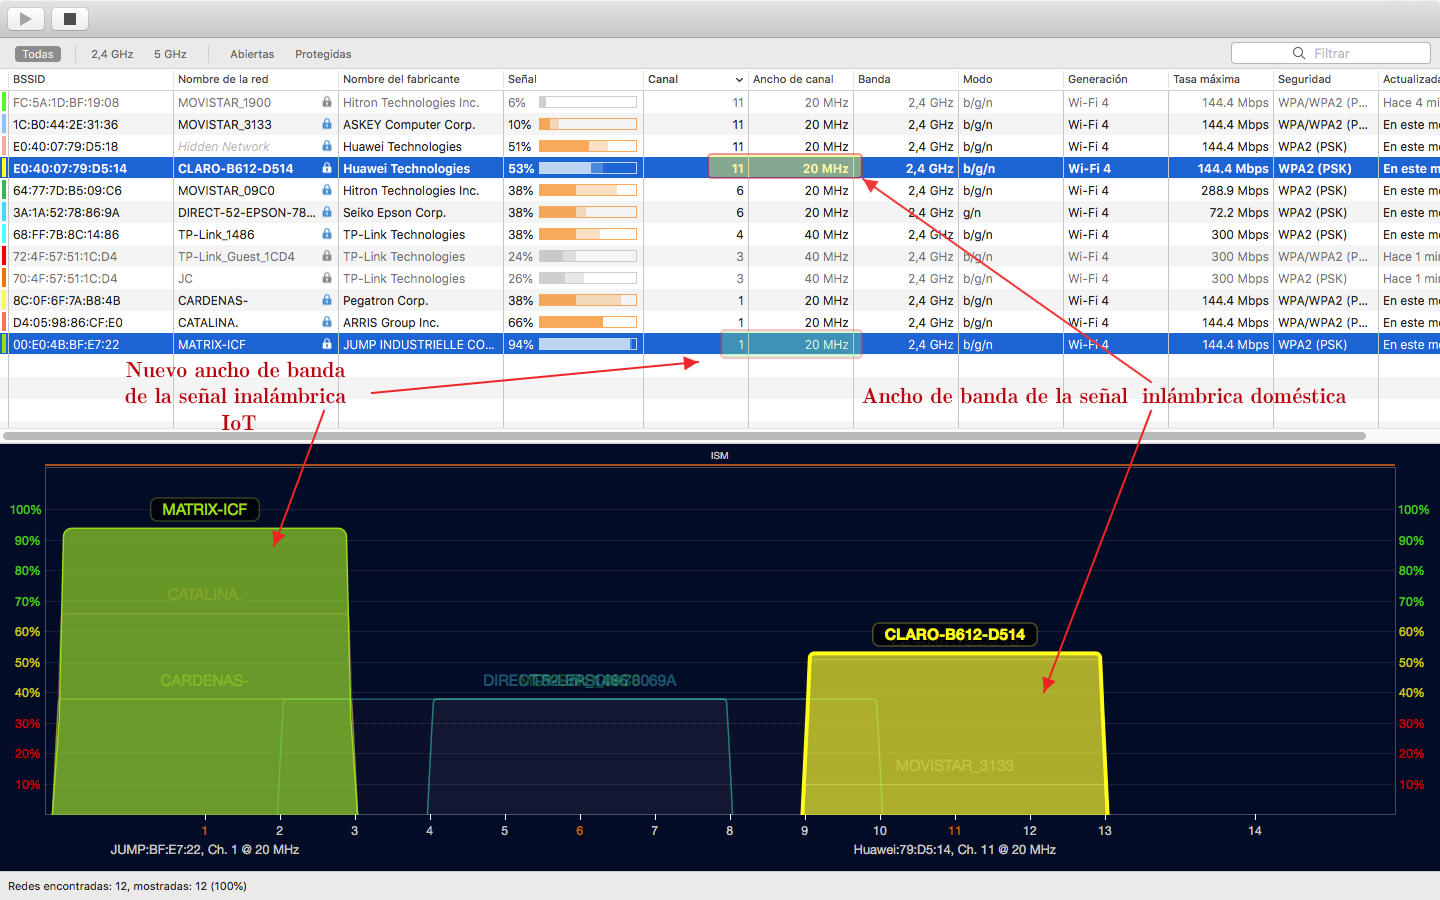
\includegraphics[width=1.5\textwidth]{./Figures/wifi/05.png}
\caption{Ancho de banda y nuevo canal de funcionamiento para las señales IoT y doméstica.}
\label{fig:test05}
\end{figure}
\end{landscape} %


%%%%%%%%%%%%%%%%%%%%%%%%%%%%%%%%%%%%%%%%%%%%%%%%%%%

\begin{landscape} % esto es para rotar la pagina e imagen
\begin{figure}[htpb]
\centering 
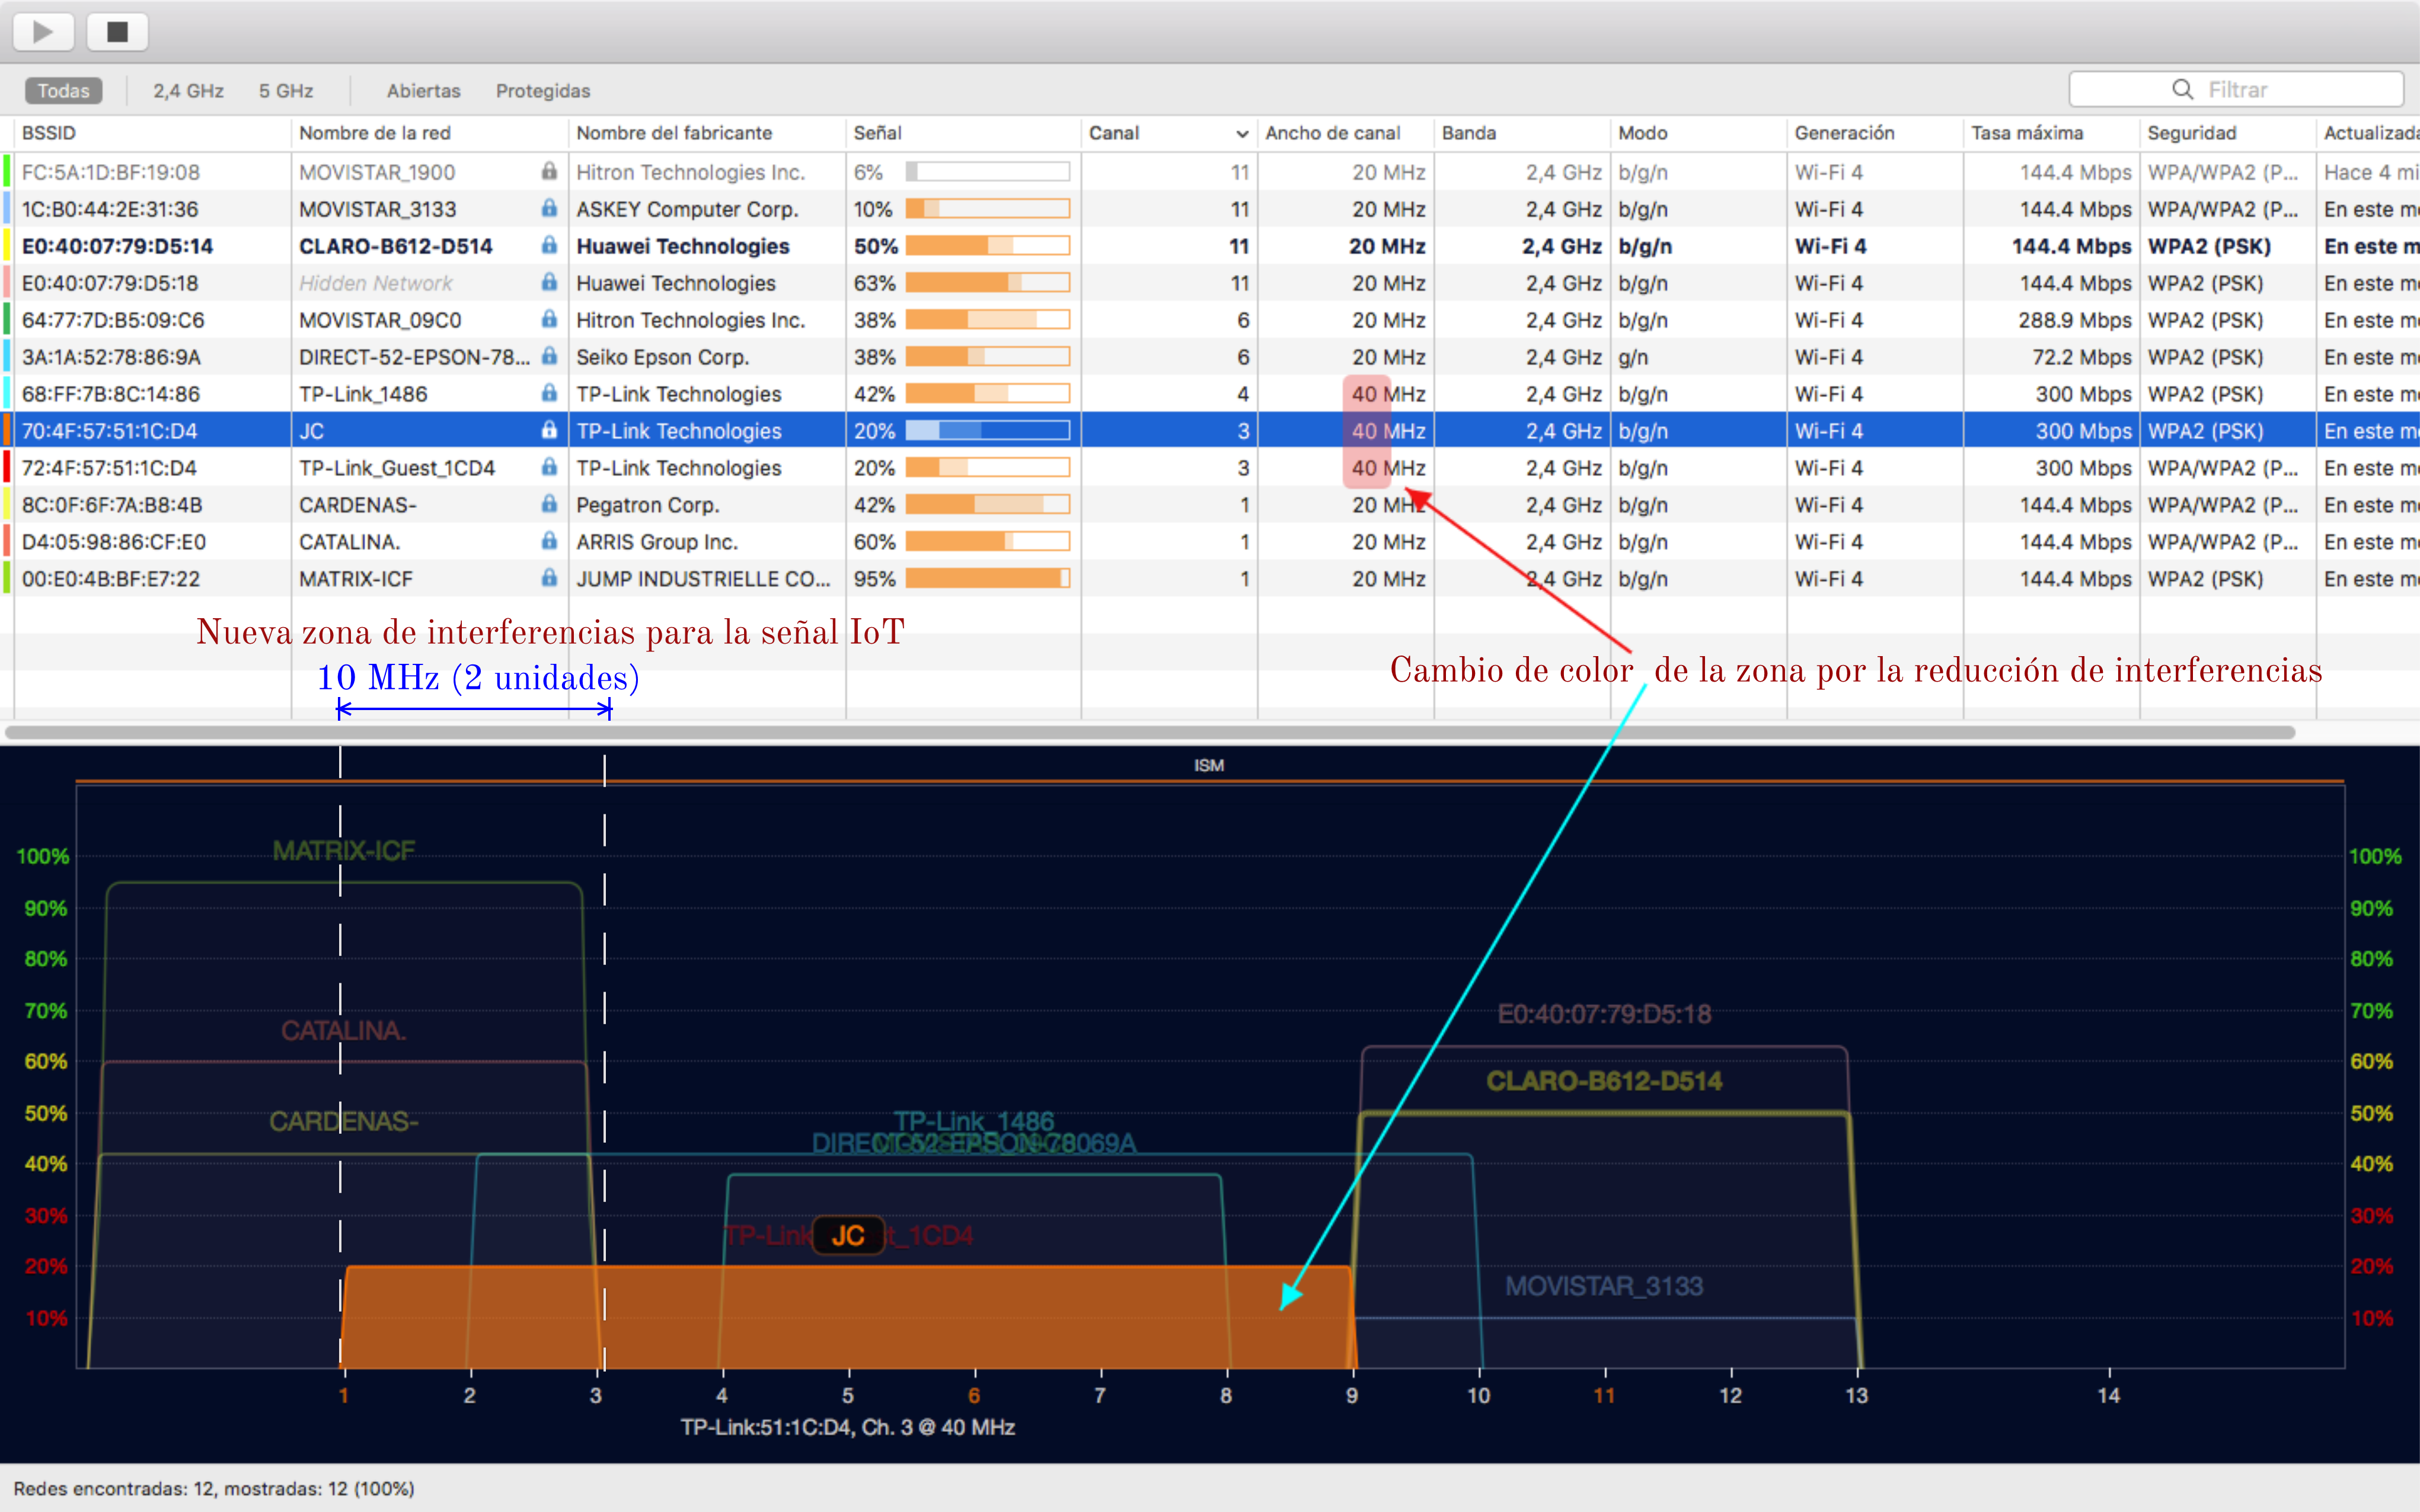
\includegraphics[width=1.5\textwidth]{./Figures/wifi/06.png}
\caption{Zona con reducción de solapamiento después de la configuración manual del router.}
\label{fig:test06}
\end{figure}
\end{landscape} %


\section{Pruebas del módulo de temperatura}
\section{Pruebas del módulo actuador y consumo}
\section{Pruebas del funcionamiento del módulo replicador}
\section{Pruebas del funcionamiento del sistema sin Internet}
\section{Pruebas y resultados de consumo de energía eléctrica}
\section{Pruebas funcionales del sistema desde acceso remoto}
